% \documentclass[12pt, twoside]{book}
\documentclass[12pt, openany, oneside]{book}

% variable values
\input variables.tex

\ifshowframe{}
    \usepackage[a4paper,top=2.5cm,bottom=2.5cm,left=3.5cm,right=2cm,showframe]{geometry}
\else
    \usepackage[a4paper,top=2.5cm,bottom=2.5cm,left=3.5cm,right=2cm]{geometry}
\fi
\usepackage{microtype}
\usepackage[slovak,USenglish]{babel}
\usepackage[utf8]{inputenc}
\usepackage[T1]{fontenc}

\linespread{1.25} % this means 1.5 line spacing

% more package imports and custom commands
\input definitions.tex

% EXPERIMENTAL: text-only mode (see `iftextonly` definition in variables.tex)
\iftextonly{}
    \renewcommand{\chapter}[2][]{}
    \renewcommand{\section}[2][]{}
    \renewcommand{\subsection}[2][]{}
    \renewcommand{\subsubsection}[2][]{}
    \renewcommand{\includegraphics}[2][]{}
    \renewcommand{\tikz}[2][]{}
    \renewcommand{\lstinputlisting}[2][]{}
    \renewcommand{\tableofcontents}{}
    \renewcommand{\footnote}{}
    \makeatletter
    \renewcommand{\th@plain}{\thm@preskip 0pt\relax\thm@postskip 0pt\relax}
    \renewcommand{\th@definition}{\thm@preskip 0pt\relax\thm@postskip 0pt\relax}
    \renewcommand{\th@remark}{\thm@preskip 0pt\relax\thm@postskip 0pt\relax}
    \makeatother
    \usepackage{enumitem}
    \setlist[enumerate]{topsep=0pt,itemsep=0pt,partopsep=0pt,parsep=0pt}
    \setlist[itemize]{topsep=0pt,itemsep=0pt,partopsep=0pt,parsep=0pt}
    \setlist[description]{topsep=0pt,itemsep=0pt,partopsep=0pt,parsep=0pt}
    \usepackage{etoolbox}
    \newcommand{\zerodisplayskips}{
    \setlength{\abovedisplayskip}{-4pt}
    \setlength{\belowdisplayskip}{-4pt}
    \setlength{\abovedisplayshortskip}{-4pt}
    \setlength{\belowdisplayshortskip}{-4pt}}
    \appto{\normalsize}{\zerodisplayskips}
    \appto{\small}{\zerodisplayskips}
    \appto{\footnotesize}{\zerodisplayskips}
    \usepackage{comment}
    \excludecomment{figure}\let\endfigure\relax
    \excludecomment{table}\let\endtable\relax
\fi

\begin{document}

\ifenglish{}
    \selectlanguage{USenglish}
\else
    \selectlanguage{slovak}
\fi

\frontmatter
\pagenumbering{gobble}

% COVER
\thispagestyle{empty}

{
    \sc\large

    \begin{center}
        \thesisuniversity{}\\
        \thesisfaculty{}

        \vfill

        \iflogoFMFI{}
            \begin{figure}[!hbt]
                \centering
                
\includegraphics[width=0.4\textwidth]{src/images/UK_Logo_BP.png}
            \end{figure}
        \fi

        {\LARGE\thesisname}\\
        \thesistype{}
    \end{center}

    \vfill

    \noindent
    \thesisyear{}\\
    \thesisauthor{}
}

\cleardoublepage{}

% TITLE PAGE
\frontmatter
\thispagestyle{empty}

\begin{center}
    \sc\large
    \thesisuniversity{}\\
    \thesisfaculty{}

    \vfill

    \iflogoFMFI{}
        \begin{figure}[!hbt]
            \centering
            
\includegraphics[width=0.4\textwidth]{src/images/FMFI_logo_BP.png}
        \end{figure}
    \fi

    {\LARGE\thesisname}\\
    \thesistype{}
\end{center}

\vfill

\noindent
\begin{tabular}{ll}
    \ifenglish{}Study Programme:\else{}Študijný program:   \fi & \thesisprogramme{}\\
    \ifenglish{}Field of Study: \else{}Študijný odbor:     \fi & \thesisfield{}\\
    \ifenglish{}Department:     \else{}Školiace pracovisko:\fi & \thesisdepartment{}\\
    \ifenglish{}Supervisor:     \else{}Školiteľ:           \fi & \thesissupervisor{}\\
    \ifconsultant{}\ifenglish{}Consultant:\else{}Konzultant:\fi & \thesisconsultant{}\\ \fi
\end{tabular}

\vfill

\noindent
\thesislocation, \thesisyear{}\\
\thesisauthor{}

\cleardoublepage{}

% ASSIGNMENT
\newpage
\thispagestyle{empty}

\noindent
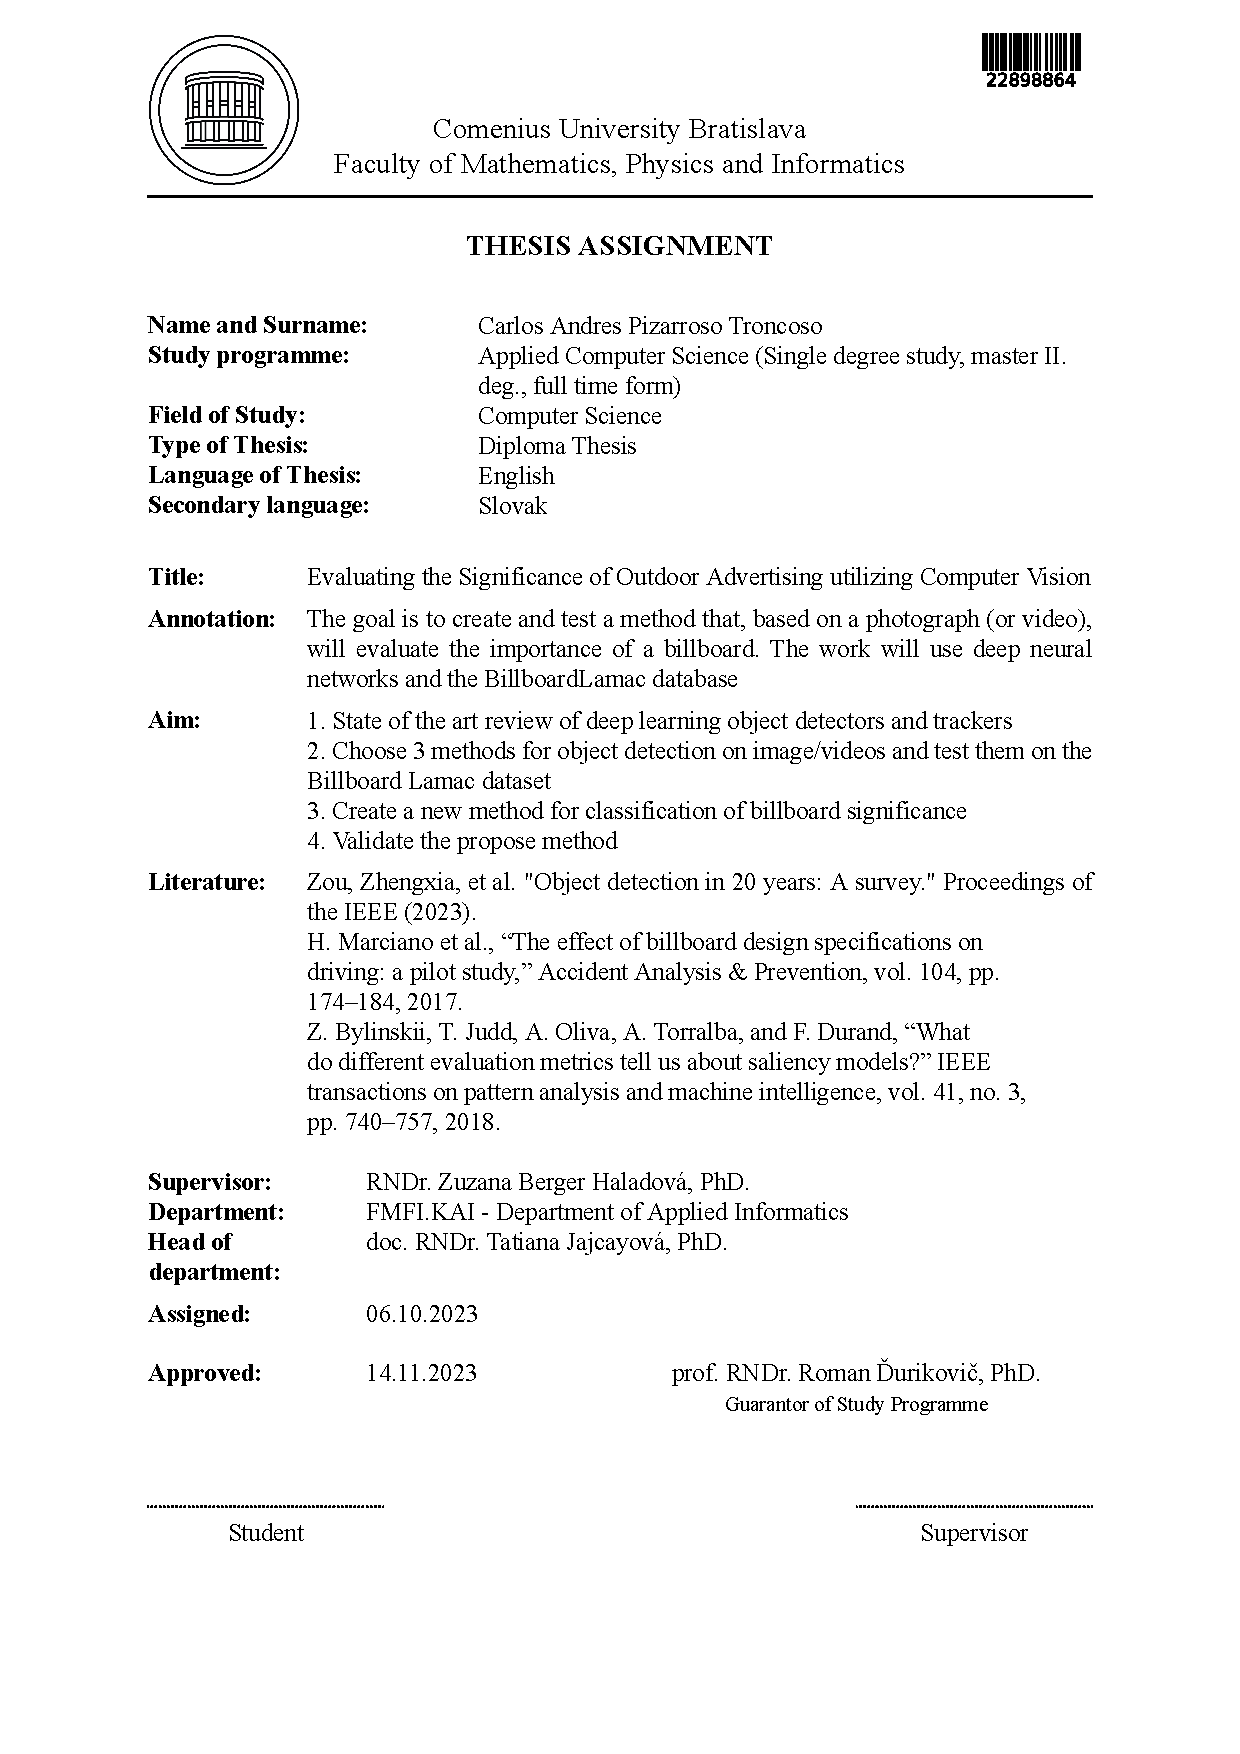
\includegraphics[trim=2.5cm 5cm 2.5cm 0,width=\textwidth]{src/documents/zadanie-zp_ENG.pdf}

\ifenglish{}
    \newpage
    \thispagestyle{empty}

    \noindent
    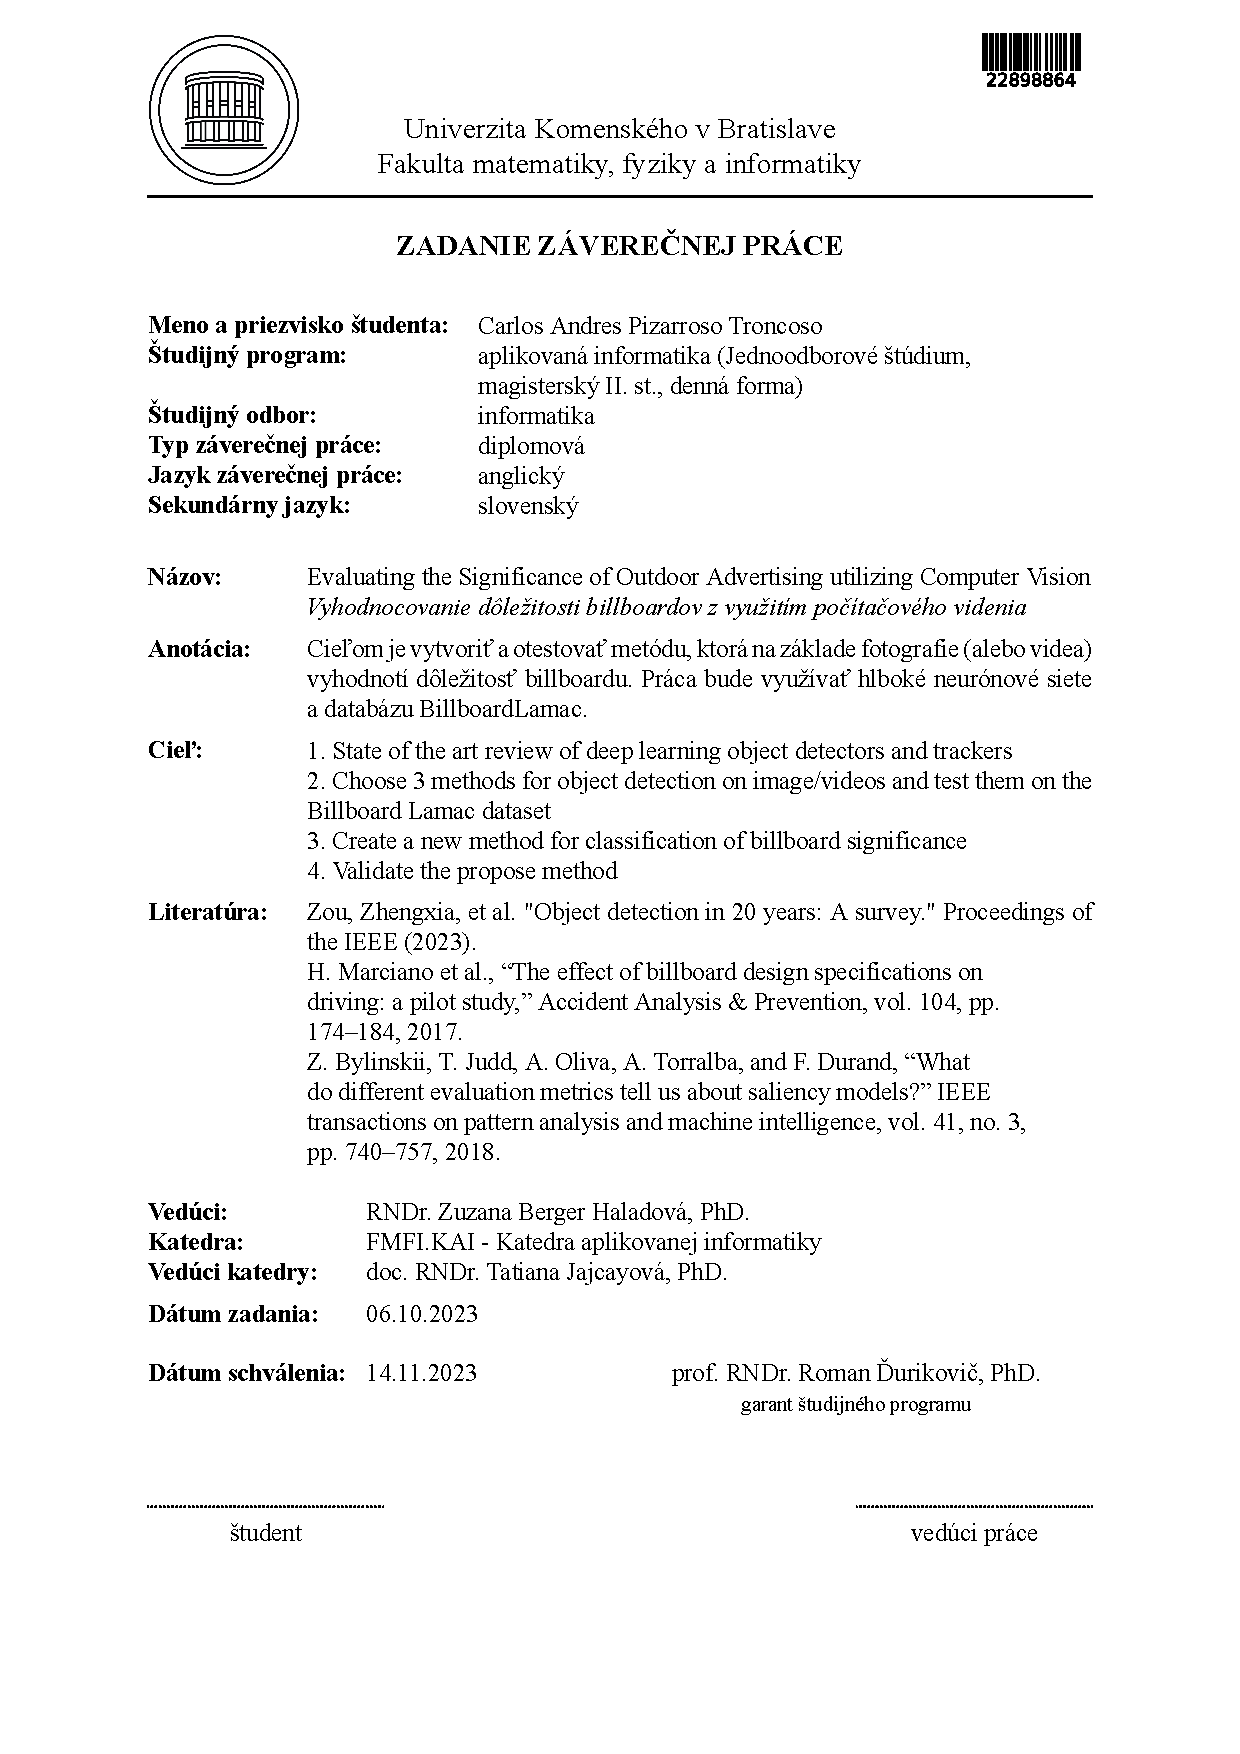
\includegraphics[trim=2.5cm 5cm 2.5cm 0,width=\textwidth]{src/documents/zadanie-zp_SK.pdf}
\fi

% ACKNOWLEDGEMENTS
\newpage

~\vfill
\paragraph*{\ifenglish{}Acknowledgments:\else{}Poďakovanie:\fi} \thesisacknowledgments{}

% ABSTRACT SK
\newpage

\begin{otherlanguage}{slovak}
    \section*{Abstrakt}

    \thesisabstractsk{Bilbordy pri cestách sú prominentným médiom vonkajšej reklamy, avšak tento typ marketingu môže potenciálne viesť k rozptýleniu počas jazdy, čím sa zvyšuje pravdepodobnosť nehôd. Na základe predchádzajúcej práce zahŕňajúcej súbor údajov BillboardLamac sa súčasná práca zameriava na výskum detekcie a klasifikácie billboardov. Aby sa to dosiahlo, bol najprv vyvinutý rámec detekcie objektov založený na YOLO s použitím podmnožiny dátového súboru Mapillary Vistas na počiatočné školenie a dátového súboru BillboardLamac na jemné doladenie. Táto metóda dosiahla spoľahlivé výsledky detekcie, čo viedlo k dvom modelom, ktoré dosiahli presnosť 93 \% a 94 \%. Okrem toho sa vyvíja snaha o klasifikáciu trvania pohľadu vodiča na billboardy, pričom sa využíva ďalšia časť súboru údajov BillboardLamac. Počiatočné štádiá vývoja klasifikátora sa zameriavajú na kategorizáciu trvania pohľadu do vopred definovaných tried. Tento prebiehajúci výskum má za cieľ prispieť k pochopeniu a prepojeniu medzi viditeľnosťou billboardov a pozornosťou vodičov, pričom sa zdôrazňuje úloha hlbokého učenia pri hodnotení vplyvu reklám na cestách.}

    \paragraph*{Kľúčové slová:} \thesiskeywordssk{slová—detekcia billboardu, detekcia objektov, modely YOLO, pozornosť vodiča, klasifikácia reklamy}
\end{otherlanguage}

% ABSTRACT EN
\newpage

\begin{otherlanguage}{USenglish}
    \section*{Abstract}

    \thesisabstracten{Roadside billboards are a prominent medium for outdoor advertisement, however, this type of marketing can potentially lead to distractions while driving, increasing the probability of accidents. Building on a previous work involving the BillboardLamac dataset, the current work aims to research into billboard detection and classification. To achieve this, a YOLO-based object detection framework was first developed, using a subset of the Mapillary Vistas dataset for initial training and the BillboardLamac dataset for fine-tuning. This method achieved reliable detection results, leading to two models which achieved 93\% and 94\% of accuracy respectively. Furthermore, an effort to classify driver gaze durations towards billboards is under development, making use of another portion of the BillboardLamac dataset. Early stages of the classifier development aim to categorize gaze durations into predefined classes. This ongoing research has the goal to contribute to the understanding and connection between billboard visibility and drivers’ attention, emphasizing the role of deep learning in evaluating roadside advertisements' impact.}

    \paragraph*{Keywords:} \thesiskeywordsen{billboard detection, object detection, YOLO models, driver attention, advertisement classification, neural networks}
\end{otherlanguage}

% TABLE OF CONTENTS, LIST OF FIGURES
\newpage
\tableofcontents

\newpage
\listoftables

\newpage
\listoffigures

% CONTENTS
\mainmatter{}
\thesischapters{}

% BIBLIOGRAPHY
\newpage
\thispagestyle{empty}
\nocite{*}
\bibliographystyle{unsrt}
\bibliography{references}

% APPENDICES
\appendix
\thesisappendices{}

\end{document}
